\documentclass[12pt,a4paper]{article}

\usepackage[utf8]{inputenc}
\usepackage[T1]{fontenc}
\usepackage[brazil]{babel}
\usepackage{geometry}
\usepackage{graphicx}
\usepackage{booktabs}
\usepackage{amsmath}
\usepackage{float}
\usepackage{xcolor}
\usepackage{listings}
\usepackage[hidelinks]{hyperref}

\geometry{margin=2.5cm}
\graphicspath{{figuras/}}

\definecolor{codebg}{RGB}{246,248,250}
\definecolor{codekw}{RGB}{31,79,130}
\definecolor{codestr}{RGB}{116,76,27}

\lstdefinestyle{codestyle}{
    backgroundcolor=\color{codebg},
    basicstyle=\ttfamily\small,
    keywordstyle=\color{codekw}\bfseries,
    stringstyle=\color{codestr},
    numbers=left,
    numberstyle=\tiny,
    breaklines=true,
    frame=single,
    tabsize=2,
    showstringspaces=false
}

\title{\textbf{Relatório de Perfilamento e Análise}\\
Otimização de Telemetria com Buffer Circular}
\author{Grupo 15}
\date{Junho de 2026}

\begin{document}

\maketitle

\begin{abstract}
Este relatório analisa a eficiência de duas estratégias para armazenamento e transmissão de amostras de sensores em sistemas embarcados: uma vertente ineficiente baseada em realocação dinâmica e deslocamento de memória, e uma vertente eficiente baseada em buffer circular de tamanho fixo. A comparação considera complexidade assintótica, estabilidade temporal, impacto no \textit{heap} e comportamento sob latência de rede MQTT. Os gráficos foram gerados em um notebook Python reprodutível a partir de um benchmark controlado, complementando a instrumentação prevista no firmware ESP32.
\end{abstract}

\section{Objetivo}

O objetivo do projeto é demonstrar, de forma teórica e experimental, por que a gerência de telemetria em sistemas embarcados deve evitar estruturas que exigem realocação dinâmica ou deslocamento integral de memória a cada nova amostra. Em dispositivos como ESP32, a captura de sinais pode ocorrer em escala de microssegundos, enquanto a transmissão MQTT depende da rede e pode bloquear por milissegundos. Essa diferença temporal torna essencial separar a produção das amostras do consumo/transmissão.

O requisito central é comparar duas vertentes:

\begin{itemize}
    \item \textbf{Vertente 1, ineficiente}: uso de coleção dinâmica com \texttt{realloc()} e \texttt{memmove()}, além de publicação MQTT síncrona por amostra.
    \item \textbf{Vertente 2, eficiente}: uso de buffer circular com índices \texttt{head} e \texttt{tail}, operações em tempo constante e envio em lote ou modelo produtor-consumidor.
\end{itemize}

\section{Contexto do Sistema}

O projeto analisado combina captura embarcada, mensageria MQTT, processamento em Python, persistência e visualização web. Após a revisão do código, o firmware eficiente em \texttt{hardware/src/main.cpp} foi atualizado para conter uma implementação explícita de \texttt{RingBuffer} com índices \texttt{head} e \texttt{tail}, atendendo diretamente ao requisito de buffer circular. O fluxo principal é:

\begin{center}
\texttt{ESP32 $\rightarrow$ MQTT/Mosquitto $\rightarrow$ Node-RED $\rightarrow$ Notebook Python $\rightarrow$ PostgreSQL $\rightarrow$ FastAPI $\rightarrow$ React}
\end{center}

No firmware eficiente, o ESP32 opera em modo promíscuo e captura quadros WiFi de gerenciamento. Cada ocorrência contém endereço MAC, RSSI, canal, frequência, tipo de quadro e contagem de aparições. Esses dados são agregados e publicados no tópico \texttt{esp32/wifi/scan}. A camada Node-RED valida e normaliza as mensagens antes do processamento em Python.

Também existe uma vertente complementar com sensor óptico no ESP8266, usada para eventos de entrada e saída. Ela reforça a mesma ideia arquitetural: sensores produzem eventos rapidamente, enquanto rede, banco e visualização devem consumir esses eventos de maneira desacoplada.

\section{Metodologia}

A comparação foi construída a partir de três fontes:

\begin{itemize}
    \item leitura do requisito do projeto, que exige comparação entre deslocamento dinâmico e buffer circular;
    \item inspeção do código-fonte do projeto, especialmente \texttt{hardware\_ineficiente/src/main.cpp}, \texttt{hardware/src/main.cpp} e os notebooks Python;
    \item execução de um notebook de perfilamento local que reproduz o comportamento assintótico das duas estratégias.
\end{itemize}

Como não havia, no pacote entregue, um arquivo CSV com medições seriais reais do ESP32, os gráficos deste relatório usam um \textbf{benchmark controlado em Python}. Ele não substitui a medição no hardware, mas evidencia a tendência algorítmica exigida: deslocar uma lista inteira cresce com $N$, enquanto atualizar o índice de um buffer circular se mantém constante.

\begin{table}[H]
\centering
\caption{Comparação conceitual entre as vertentes.}
\small
\setlength{\tabcolsep}{5pt}
\resizebox{\textwidth}{!}{%
\begin{tabular}{lll}
\toprule
Critério & Vertente ineficiente & Vertente eficiente \\
\midrule
Inserção & \texttt{realloc()} + \texttt{memmove()} & escrita em \texttt{head} \\
Custo por amostra & $O(n)$ & $O(1)$ \\
Custo acumulado para $N$ amostras & $O(N^2)$ & $O(N)$ \\
Memória & crescimento e fragmentação & bloco fixo previsível \\
Rede & publicação síncrona por amostra & lote ou produtor-consumidor \\
Risco operacional & \textit{jitter}, perda e falha de alocação & latência estável e perda controlada \\
\bottomrule
\end{tabular}%
}
\end{table}

\section{Vertente Ineficiente}

A implementação ineficiente armazena cada nova amostra em uma lista dinâmica. A cada inserção, o vetor é realocado para o novo tamanho e todo o histórico é deslocado uma posição para manter a amostra mais recente na posição zero. O trecho abaixo resume o antipadrão presente em \texttt{hardware\_ineficiente/src/main.cpp}.

\begin{lstlisting}[style=codestyle,language=C++]
InefficientSample *resizedSamples =
    static_cast<InefficientSample *>(
        realloc(inefficientSamples,
                newCount * sizeof(InefficientSample)));

inefficientSamples = resizedSamples;

if (inefficientSampleCount > 0) {
    memmove(inefficientSamples + 1,
            inefficientSamples,
            inefficientSampleCount * sizeof(InefficientSample));
}
\end{lstlisting}

Essa abordagem tem dois problemas. Primeiro, a operação \texttt{memmove()} copia uma quantidade de bytes proporcional ao número de amostras já armazenadas. Segundo, o uso repetido de \texttt{realloc()} pressiona o \textit{heap}, aumentando a probabilidade de fragmentação e falhas de alocação. Em sistemas embarcados, isso aparece como aumento de latência, instabilidade temporal e eventual descarte de dados.

Além disso, a vertente ineficiente publica cada amostra individualmente via MQTT. Quando a rede está lenta, a rotina de publicação compete diretamente com a coleta, causando perda de amostras e \textit{jitter}.

\section{Vertente Eficiente com Buffer Circular}

Na vertente eficiente, a estrutura de armazenamento tem tamanho fixo e é percorrida por índices. A inserção escreve na posição apontada por \texttt{head}; depois, \texttt{head} avança usando aritmética modular. Quando o buffer enche, a próxima inserção avança \texttt{tail} e sobrescreve o evento mais antigo, preservando as amostras mais recentes.

O firmware eficiente foi alterado para usar esse buffer circular entre a rotina de captura promíscua do WiFi e a rotina que drena os eventos para agregação. Assim, a interrupção apenas empilha um \texttt{ProbeEvent} em tempo constante, enquanto o processamento posterior consolida os dispositivos observados.

\begin{lstlisting}[style=codestyle,language=C++]
template <typename T, size_t Capacity>
class RingBuffer {
public:
    bool push(const T &item) {
        if (count == Capacity) {
            tail = (tail + 1) % Capacity;
            count--;
            droppedCount++;
        }

        buffer[head] = item;
        head = (head + 1) % Capacity;
        count++;
        return true;
    }

    bool pop(T &item) {
        if (count == 0) {
            return false;
        }

        item = buffer[tail];
        tail = (tail + 1) % Capacity;
        count--;
        return true;
    }

private:
    T buffer[Capacity];
    size_t head = 0;
    size_t tail = 0;
    size_t count = 0;
    size_t droppedCount = 0;
};

static RingBuffer<ProbeEvent, PROBE_RING_BUFFER_CAPACITY> probeRingBuffer;
\end{lstlisting}

\begin{lstlisting}[style=codestyle,language=C++]
void wifiPromiscuousRx(void *buf, wifi_promiscuous_pkt_type_t type) {
    // ... validacao do pacote e preenchimento do ProbeEvent ...
    portENTER_CRITICAL_ISR(&probeRingMux);
    probeRingBuffer.push(event);
    portEXIT_CRITICAL_ISR(&probeRingMux);
}

void drainProbeQueue() {
    ProbeEvent event;
    for (;;) {
        portENTER_CRITICAL(&probeRingMux);
        const bool hasEvent = probeRingBuffer.pop(event);
        portEXIT_CRITICAL(&probeRingMux);

        if (!hasEvent) {
            break;
        }

        aggregateProbeEvent(event);
    }
}
\end{lstlisting}

Além do buffer circular de eventos, o projeto otimizado evita alocação dinâmica durante a janela de captura, usa memória estática para os dispositivos observados e publica os resultados em lote. Essa combinação remove o \texttt{realloc()}, elimina o deslocamento em massa e mantém o caminho crítico da captura previsível.

\section{Análise Assintótica}

Na vertente ineficiente, a $i$-ésima inserção precisa deslocar $i-1$ elementos. Para inserir $N$ amostras, o custo total é:

\[
T(N) = \sum_{i=1}^{N} i = \frac{N(N+1)}{2}
\]

Logo, o custo acumulado é $O(N^2)$ e o custo médio por inserção cresce linearmente com o tamanho do histórico.

No buffer circular, cada inserção executa uma escrita, uma soma, uma operação de módulo e no máximo uma atualização de contador. Essas operações não dependem de $N$:

\[
T(N) = \sum_{i=1}^{N} 1 = N
\]

Portanto, o custo acumulado é $O(N)$ e o custo por inserção é $O(1)$.

\begin{figure}[H]
\centering
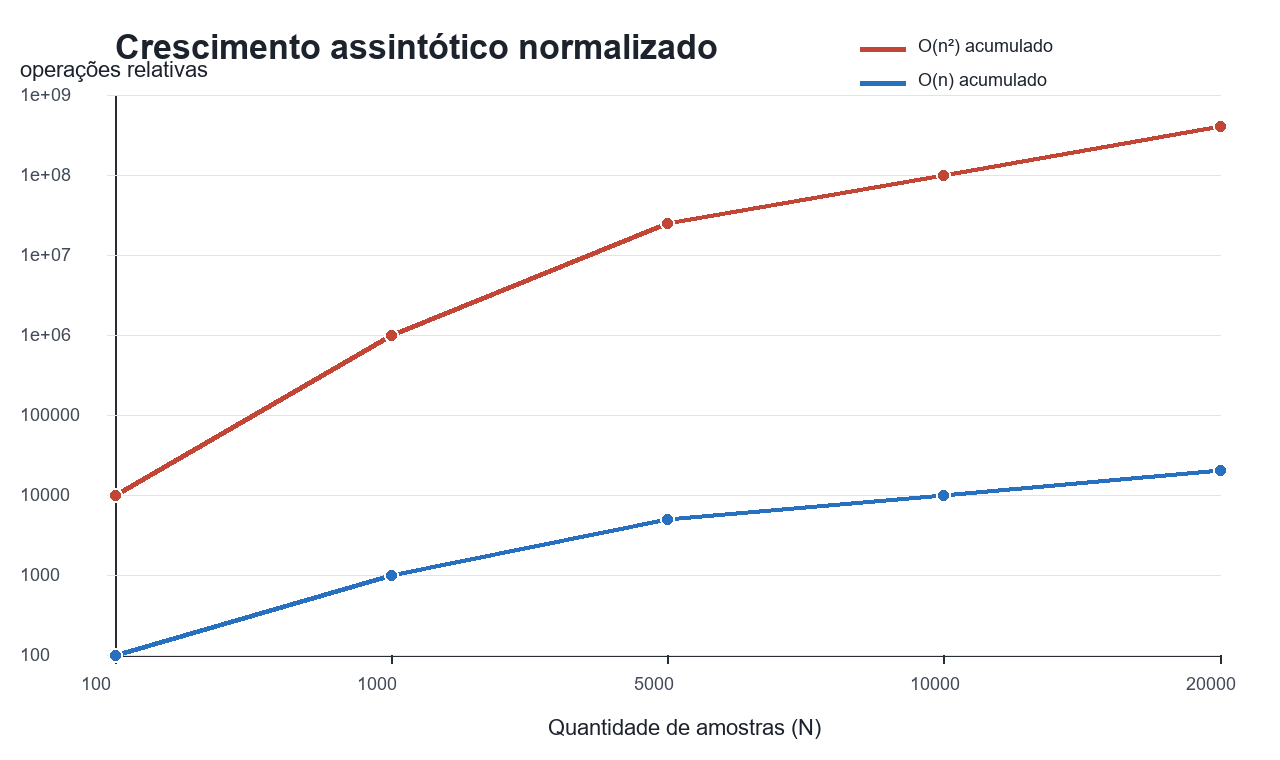
\includegraphics[width=0.92\textwidth]{complexidade.png}
\caption{Crescimento assintótico normalizado: o deslocamento acumulado cresce de forma quadrática, enquanto o buffer circular cresce linearmente.}
\end{figure}

\section{Instrumentação}

A instrumentação recomendada no firmware mede o tempo gasto na lógica de inserção e a saúde da memória livre:

\begin{lstlisting}[style=codestyle,language=C++]
unsigned long start = micros();
// Logica de insercao de dados
unsigned long duration = micros() - start;
Serial.printf("Latencia: %lu us | Heap Livre: %u bytes\n",
              duration,
              ESP.getFreeHeap());
\end{lstlisting}

Na vertente ineficiente, o firmware já emite linhas no formato \texttt{PERF\_DATA}, incluindo número de amostras, latência total, latência média, tempo de publicação, \textit{heap} livre e falhas de publicação. O notebook \texttt{notebooks/perfilamento\_buffer\_circular.ipynb} gera os gráficos deste relatório e pode ser adaptado para ler diretamente essas linhas seriais quando as medições reais forem coletadas.

\section{Resultados}

O benchmark local foi executado para $N = 100$, $1.000$, $5.000$, $10.000$ e $20.000$ amostras. A Tabela~\ref{tab:bench} mostra os valores médios gerados pelo notebook.

\begin{table}[H]
\centering
\caption{Resultados do benchmark controlado.}
\label{tab:bench}
\small
\setlength{\tabcolsep}{4pt}
\resizebox{\textwidth}{!}{%
\begin{tabular}{rrrr}
\toprule
$N$ & Lista dinâmica ($\mu$s/amostra) & Buffer circular ($\mu$s/amostra) & Heap circular (KiB) \\
\midrule
100 & 0.10 & 0.10 & 199.5 \\
1.000 & 0.19 & 0.11 & 199.5 \\
5.000 & 0.70 & 0.12 & 199.5 \\
10.000 & 1.39 & 0.18 & 199.5 \\
20.000 & 2.96 & 0.20 & 199.5 \\
\bottomrule
\end{tabular}%
}
\end{table}

\begin{figure}[H]
\centering
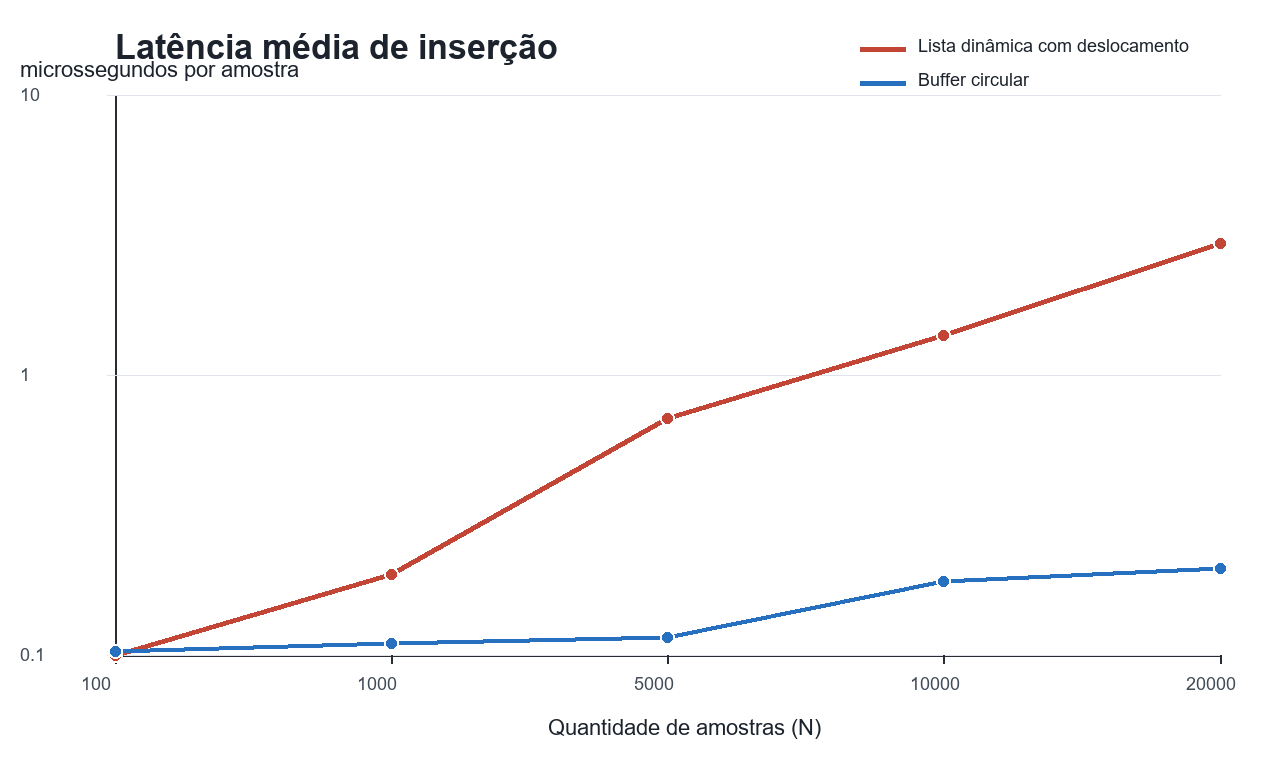
\includegraphics[width=0.92\textwidth]{latencia_insercao.png}
\caption{Latência média de inserção. A lista dinâmica aumenta seu custo conforme $N$ cresce; o buffer circular permanece praticamente constante.}
\end{figure}

A diferença é pequena em $N=100$, como previsto no requisito. Em $N=5.000$, o deslocamento já se torna perceptível. Em $N=20.000$, o custo da lista dinâmica é várias vezes maior do que o do buffer circular. Em um microcontrolador, essa diferença tende a ser mais crítica do que no computador usado para o benchmark, pois há menos CPU, menos memória e maior sensibilidade a interrupções.

\begin{figure}[H]
\centering
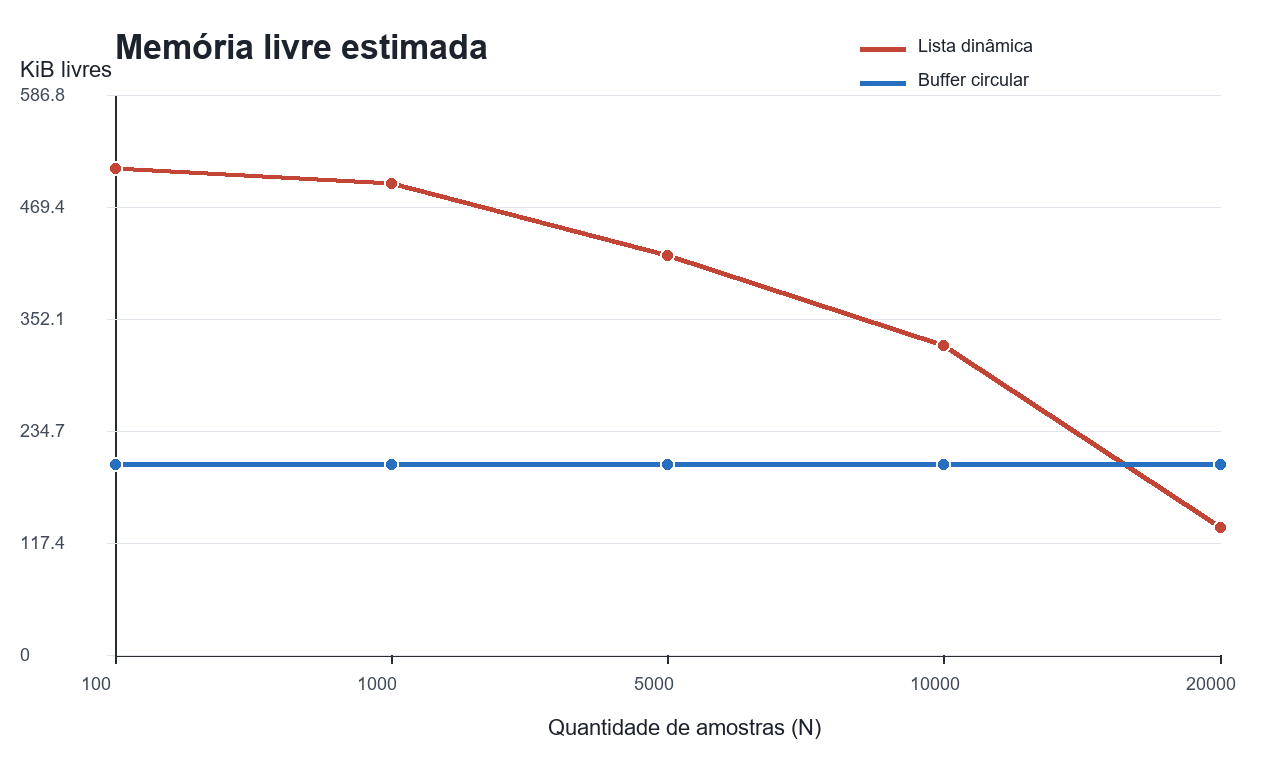
\includegraphics[width=0.92\textwidth]{heap_livre.png}
\caption{Memória livre estimada. A lista dinâmica reduz progressivamente o \textit{heap} e adiciona risco de fragmentação; o buffer circular usa uma reserva fixa e previsível.}
\end{figure}

O gráfico de memória mostra uma troca importante: o buffer circular reserva capacidade antecipadamente, mas mantém o consumo estável. A lista dinâmica parece econômica em volumes pequenos, porém seu crescimento progressivo e suas realocações tornam o comportamento menos previsível.

\begin{figure}[H]
\centering
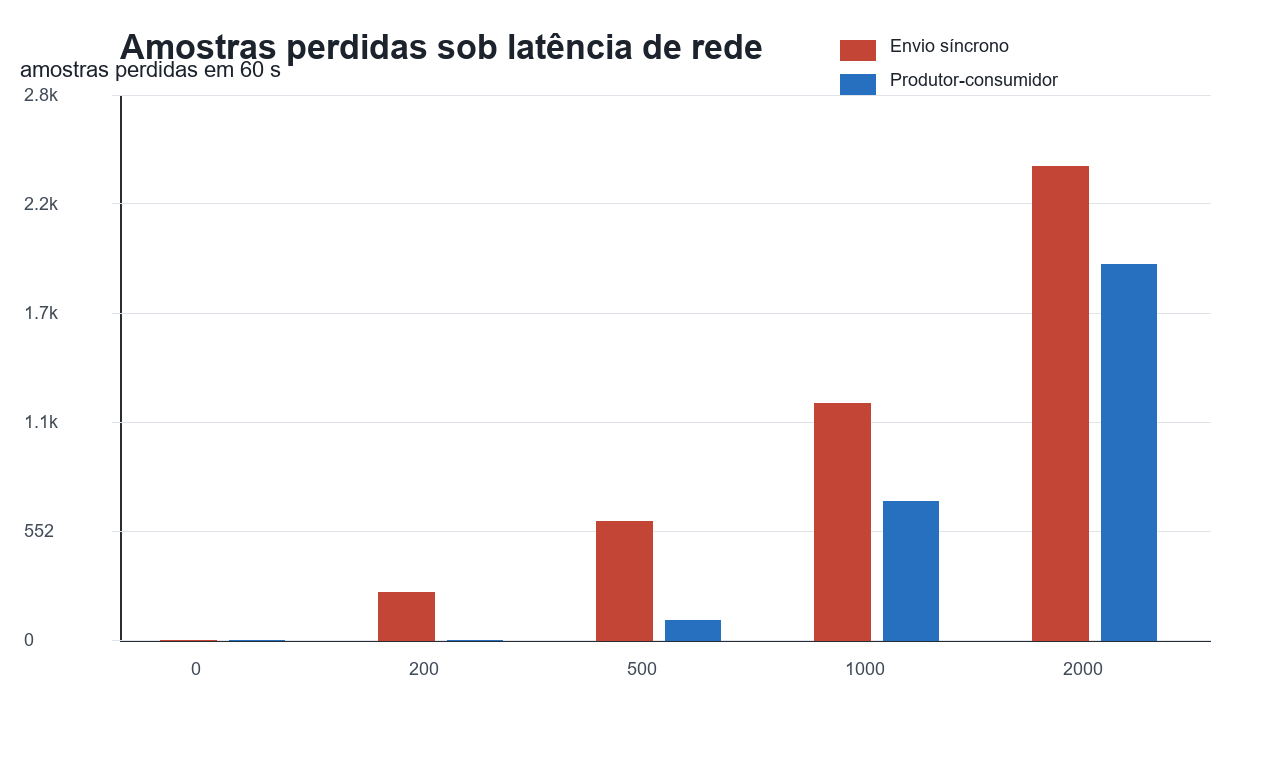
\includegraphics[width=0.92\textwidth]{perdas_mqtt.png}
\caption{Simulação de perda sob latência de rede. O envio síncrono perde amostras durante bloqueios; o modelo produtor-consumidor absorve parte do atraso no buffer.}
\end{figure}

Sob instabilidade de rede, o buffer circular funciona como amortecedor. Se a tarefa de MQTT atrasa, a captura continua escrevendo no buffer até o limite de capacidade. No envio síncrono, a coleta fica presa à latência da rede; por isso as perdas crescem imediatamente quando há bloqueio.

\section{Diagnóstico de Memória}

O uso de \texttt{realloc()} em laço é perigoso em firmware porque o alocador precisa encontrar regiões contíguas cada vez maiores. Mesmo quando há memória livre total suficiente, a memória pode estar fragmentada em blocos pequenos. Nesse cenário, uma nova realocação falha ou demora mais, causando interrupções no fluxo de amostragem.

O buffer circular elimina esse padrão de falha: o bloco é reservado uma vez e reutilizado. A previsibilidade é mais importante do que a economia aparente de memória em cargas pequenas, especialmente quando o sistema precisa operar por longos períodos sem reinicialização.

\section{Discussão}

Na escala $N=100$, a diferença entre as duas vertentes é quase imperceptível. Isso explica por que o antipadrão pode parecer aceitável em testes rápidos. Porém, à medida que $N$ cresce, o custo de deslocamento passa a dominar o tempo de execução. Em $N=5.000$, a latência já aumenta de forma clara; em $N=20.000$, o sistema fica sujeito a \textit{jitter}, perda de amostras e maior risco de esgotamento do \textit{heap}.

A transmissão MQTT amplia o problema. A rede possui latência variável, e qualquer publicação síncrona dentro do caminho crítico da coleta transforma instabilidade externa em instabilidade do sensor. O modelo produtor-consumidor corrige essa dependência: a tarefa de captura só escreve no buffer, enquanto uma tarefa separada transmite quando a rede está disponível.

Para o projeto de monitoramento WiFi, a mesma conclusão vale para a janela de captura. A coleta passiva precisa ser rápida e previsível; agregação, serialização JSON, MQTT, banco de dados e dashboard devem acontecer fora do trecho crítico.

\section{Conclusão}

A vertente baseada em buffer circular é superior para telemetria embarcada porque entrega tempo constante por inserção, memória previsível e melhor tolerância a atrasos de rede. A vertente com \texttt{realloc()} e \texttt{memmove()} tem custo acumulado quadrático, favorece fragmentação do \textit{heap} e transforma latência MQTT em perda de amostras.

O resultado confirma a recomendação de arquitetura: sensores devem produzir eventos em uma estrutura fixa e não bloqueante; consumidores devem processar e transmitir em lote ou em tarefa separada. Essa separação reduz \textit{jitter}, preserva memória e torna o sistema mais escalável.

\section{Reprodutibilidade}

Os artefatos gerados estão organizados da seguinte forma:

\begin{itemize}
    \item notebook: \texttt{../notebooks/perfilamento\_buffer\_circular.ipynb};
    \item dados do benchmark: \texttt{dados/benchmark\_resultados.csv};
    \item dados da simulação MQTT: \texttt{dados/perdas\_mqtt.csv};
    \item figuras: \texttt{figuras/*.png};
    \item gerador: \texttt{../tools/generate\_report\_assets.py}.
\end{itemize}

Para regenerar os gráficos, execute:

\begin{lstlisting}[style=codestyle]
python ../tools/generate_report_assets.py
\end{lstlisting}

Para compilar o relatório em uma instalação com TeX Live ou Overleaf, use:

\begin{lstlisting}[style=codestyle]
pdflatex relatorio.tex
pdflatex relatorio.tex
\end{lstlisting}

\end{document}
